
Transformers are predominantly utilized in generating text for Large Language Models (LLMs) like GPT \autocite{GPT2radford2019} and LaMMA \autocite{touvron2023llama}. This thesis aims to explore the application of conventional Transformer-based architectures for the generation of texture assets, diverging from the traditional image generation methods primarily relying on stable diffusion techniques or Generative Adversarial Networks (GANs).

To achieve this, three distinct models are developed and trained, each incorporating unique modifications to harness the principal benefits of Transformer-based models for image texture generation. The dataset required for training these models is compiled from a variety of sources, necessitating thorough cleaning and analysis to ensure usability. The objective is for these trained models to be capable of generating basic floor textures suitable for use as assets in video games. These developed models are compared using a specific set of metrics. Furthermore, the development process will be briefly outlined, highlighting the differences from conventional programming workflows typically encountered.



\subsection{Related work}
    
The exploration of machine learning models for image generation has been a significant area of research lately, with notable advancements from Generative Adversarial Networks (GANs) to state-of-the-art diffusion models. This section reviews the seminal works and recent innovations in the field, particularly focusing on image/texture generation and the application of Transformer models in the context of images, laying the foundation for the current study's approach to image generating.

\textbf{Generative Adversarial Networks (GANs):} 
Since their introduction by \autocite{goodfellow2014generative}, GANs have been a cornerstone in the field of generative models, especially for image generation tasks. Works by \autocite{radford2016unsupervised}, introducing the DCGAN architecture, demonstrated the potential of GANs in producing high-quality images. The adaptability of GANs has been explored in various contexts, including texture synthesis \autocite{xian2018texturegan}, showcasing their capability to generate seamless textures for different materials.

\textbf{Diffusion Models:} 
Diffusion models represent a cutting-edge development in the field of generative models, that demonstrate remarkable capabilities in image generation by iterative denoising a random signal to produce detailed images. The process, initially introduced by \autocite{sohldickstein2015deep}, involves gradually adding noise to an image across several steps and then learning to reverse this process. Stable diffusion, a term often associated with these models, refers to the technique's ability to maintain stability throughout the noise addition and removal process, ensuring high-quality image synthesis. The paper \enquote{Diffusion Models Beat GANs on Image Synthesis} \autocite{dhariwal2021diffusion} further refined this concept with models like DDPM, showcasing exceptional fidelity in generated images. This approach contrasts traditional models by focusing on the controlled removal of noise, leading to the generation of coherent and visually impressive images.

\textbf{Transformers in Image classification:} 
The success of Transformer models in natural language processing, as seen with architectures like GPT \autocite{GPT2radford2019} and LaMMA \autocite{touvron2023llama}, has inspired their application in image-related tasks. The Vision Transformer (ViT) by \autocite{dosovitskiy2021image} marked a significant leap, applying Transformers directly to sequences of image patches for classification tasks. This idea was extended to image generation through architectures like the VideoGPT by \autocite{yan2021videogpt}, which demonstrated that Transformer models could generate coherent and detailed videos.

\textbf{Texture Generation with Transformers:}
TransGAN by \autocite{jiang2021transgan} revolutionizes image generation with a Transformer-based GAN architecture, moving beyond traditional CNN approaches. It features a memory-efficient generator and a nuanced, multiscale discriminator, both utilizing transformer blocks. With advanced training techniques to overcome common GAN challenges, TransGAN produces high-quality images, showcasing the potential of Transformers in this new domain.

\subsection{Infrastructure for Model Development}

To develop and train the models in this thesis, a powerful computing infrastructure is necessary to manage the extensive datasets and the substantial computational requirements for model training. Unlike conventional development environments where a standard laptop or desktop may suffice, most of the models in this thesis demand a more capable infrastructure. Therefore, a high-performance computing system situated in Berlin is used for the model training processes. This system contains an array of (NVIDIA Tesla A100 80 GB) GPUs, (INTEL Ice Lake 8360Y) CPUs and a significant quantity of RAM. Such a configuration, especially the substantial GPU memory, enables the training and execution of larger models that would be possible on a home workstation. The development of these models is carried out using Python and PyTorch, with the code being crafted in Visual Studio Code and managed through version control with Git. The model development and initial code testing are done on a local machine, reserving the high-performance system exclusively for the final training phases. This approach diverges from standard practices, where often both development and execution occur on the same development platform. Ensuring the code is free of errors prior to giving the task of training the model to the high-performance computing system is crucial, as discovering bugs in the training process can be exceedingly time-consuming. For instance, to endure a training session that extends for 30 hours, only to realize it terminated prematurely due to script errors.

\subsection{Data}
    
This section describes the methods used for gathering, cleaning, and analyzing data in a research thesis on textures. Essential for training a machine learning model, the data is carefully collected from various sources, cleaned to maintain uniformity, and examined for patterns, with a focus on color distribution.


\subsubsection{Data Retrieval}
On the internet, a wide variety of textures can be found, but not all of them are suitable for this task. The textures should be seamless, devoid of shadows, and free from any objects. Textures of floors, such as carpets, tiles, wood, concrete, and more, were utilized. Two approaches were employed to acquire the data for this thesis.

\begin{itemize}
    \item Web Data Collection

    The data for this project was obtained from various online sources. Numerous free texture providers, such as textures.com, texturehaven.com, and others, were utilized for data acquisition. Due to the limitation of downloading one texture at a time from most websites, a series of scripts were developed to compile a list of suitable textures and automate the downloading process. These scripts were created using UiPath and Python.
    
    \item Video Game Textures
    
    The second approach involved using textures from video games. The advantage of this approach is that these textures are already seamless and often of high quality and quantity. However, a drawback is that these textures can be very repetitive. To obtain these textures, downward-facing recordings of the game were made, and the textures were extracted from the video. The major challenge with this approach is the need to disable shadows and all UI elements (HUD elements) in the game, which is not always possible.
\end{itemize}

\subsubsection{Data Cleaning}

    To ensure that the data is consistent and free from elements that could corrupt the model, various cleaning steps were applied. For example, all images containing 3D objects were removed, especially those gathered from video games. During the recording of the floor, unwanted debris or pieces of wood were often present, and all extracted frames were manually checked.

    In the case of web-gathered textures, there were different folder structures, and it was necessary to standardize them across all data folders. Additionally, some of them had associated files that were irrelevant to this use case and needed to be discarded.

    All the images were in high-definition (HD) quality, with a height of approximately 1024 pixels.


    \begin{table}[h]
        \centering
        \begin{tabular}{|c|c|c|}
            \hline
            Dataset & Size & Number of Images \\
            \hline
            Free PBR & 452.0 MB & 263 \\
            Polyhaven & 298.0 MB & 439 \\
            Poliigon & 70.4 MB & 49 \\
            Minecraft-Textures &  636.0 MB & 493 \\
            CsGoFloor-Textures & 18.3 GB & 44540 \\
            \hline
            Combined & 20.2 GB & 45784 \\
            \hline
        \end{tabular}
        \caption{Datasets collected for this thesis}
        \label{tab:datasets}
    \end{table}

    \subsubsection{Patterns in the data}
    
    To examine whether the dataset encompasses a broad spectrum of colors, multiple plots are created. These plots illustrate the color distribution within the datasets, providing insights into the diversity of colors present. Prior to plotting, a comprehensive pixel count across all images is conducted. For instance, if an image features 10 pixels of the color $(255, 0, 0)$, this count is added to a dictionary. Should the subsequent image in the dataset contain 5 pixels of the same color, these are also incorporated into the dictionary, cumulating a total of 15 for that specific color. This process is repeated for each color encountered, aggregating the counts to yield the overall color frequency within the dataset.

\begin{lstlisting}[language=Python]
  color_counts = {} 
  for i, (data, _) in enumerate(dataset):
      # data is a tensor of shape (3, height, width) 
      pixel_rgb_array = (data.view(3, -1).t() * 255).to(torch.int32)
      
      for pixel_color in map(tuple, pixel_rgb_array):
          if color in color_counts:
              color_counts[pixel_color] += 1
          else:
              color_counts[pixel_color] = 1
\end{lstlisting}

    After analyzing the dataset through this method, visual representations of the color distributions were produced using Python and Matplotlib. These plots provide a three-dimensional view of the RGB color space, where the X, Y, and Z axes correspond to the Red, Green, and Blue color values, respectively, each ranging from 0 to 255. 

    \[
    \text{size} = \log(\text{count of color}) \times 20
    \]

    The size of each plotted point is calculated based on the logarithm of the color count, scaled by a factor of 20.
    
    

    \begin{figure}[h]
        \centering
        
        \begin{subfigure}{.33\textwidth}
          \centering
          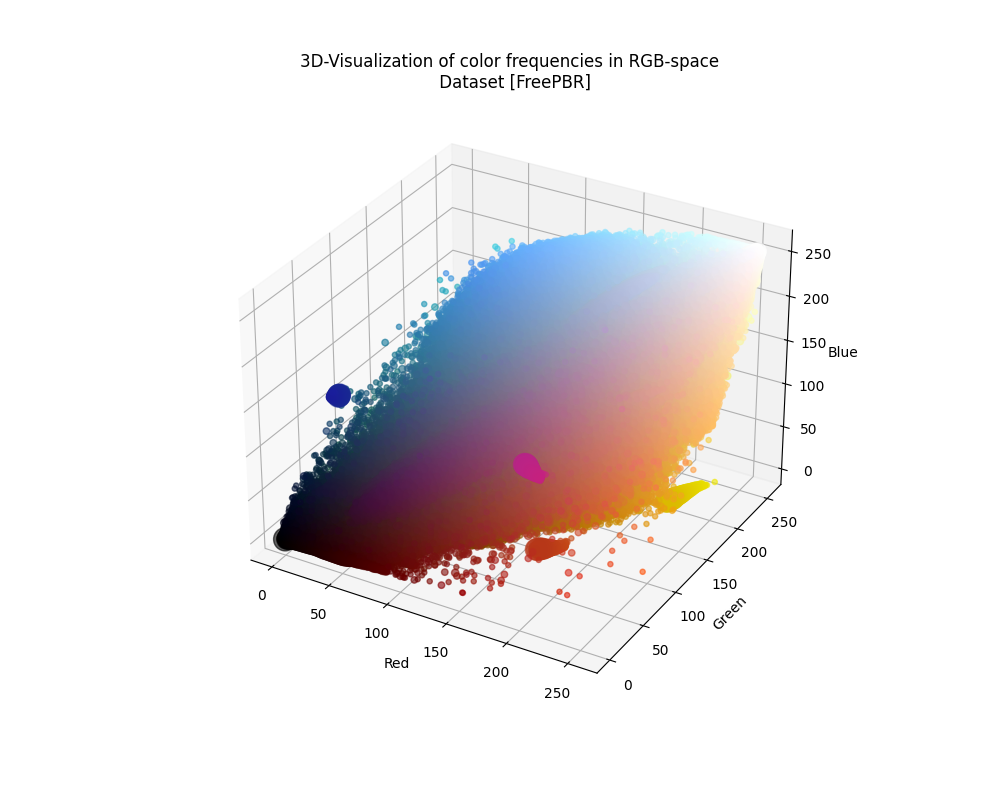
\includegraphics[width=\linewidth]{../code/dataAnalysis/output/FreePBR.png}
          \caption{FreePBR}
          \label{fig:dataset-FreePBR}
        \end{subfigure}%
        \hfill
        \begin{subfigure}{.33\textwidth}
          \centering
          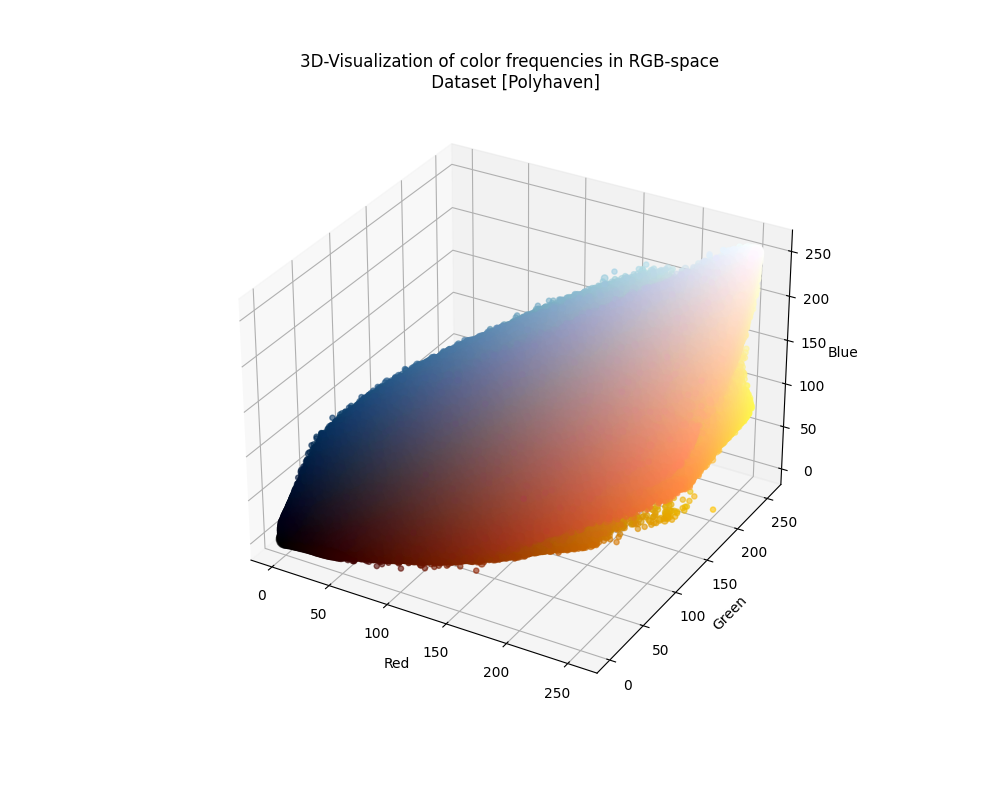
\includegraphics[width=\linewidth]{../code/dataAnalysis/output/Polyhaven.png}
          \caption{Polyhaven}
          \label{fig:dataset-Polyhaven}
        \end{subfigure}%
        \hfill
        \begin{subfigure}{.33\textwidth}
          \centering
          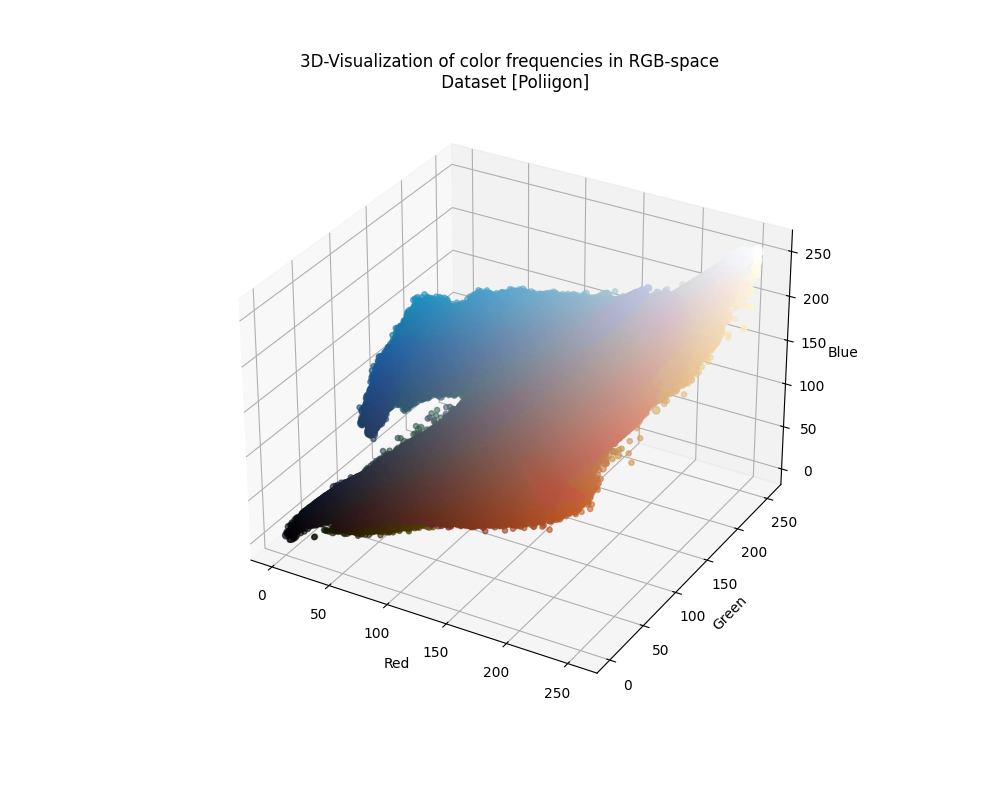
\includegraphics[width=\linewidth]{../code/dataAnalysis/output/Poliigon.png}
          \caption{Poliigon}
          \label{fig:dataset-Poliigon}
        \end{subfigure}
        
        \vspace{1cm} % Vertikaler Abstand zwischen den Reihen
        
        \begin{subfigure}{.33\textwidth}
          \centering
          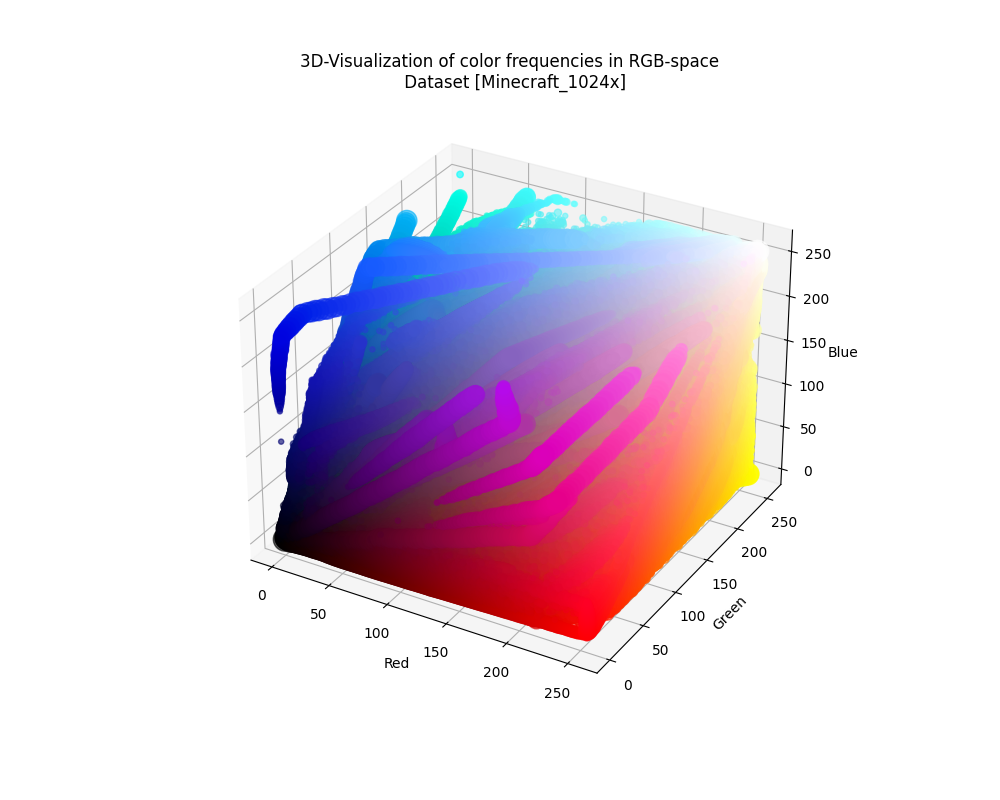
\includegraphics[width=\linewidth]{../code/dataAnalysis/output/Minecraft_1024x.png}
          \caption{Minecraft-Textures}
          \label{fig:dataset-Minecraft-Textures}
        \end{subfigure}%
        \hfill
        \begin{subfigure}{.33\textwidth}
          \centering
          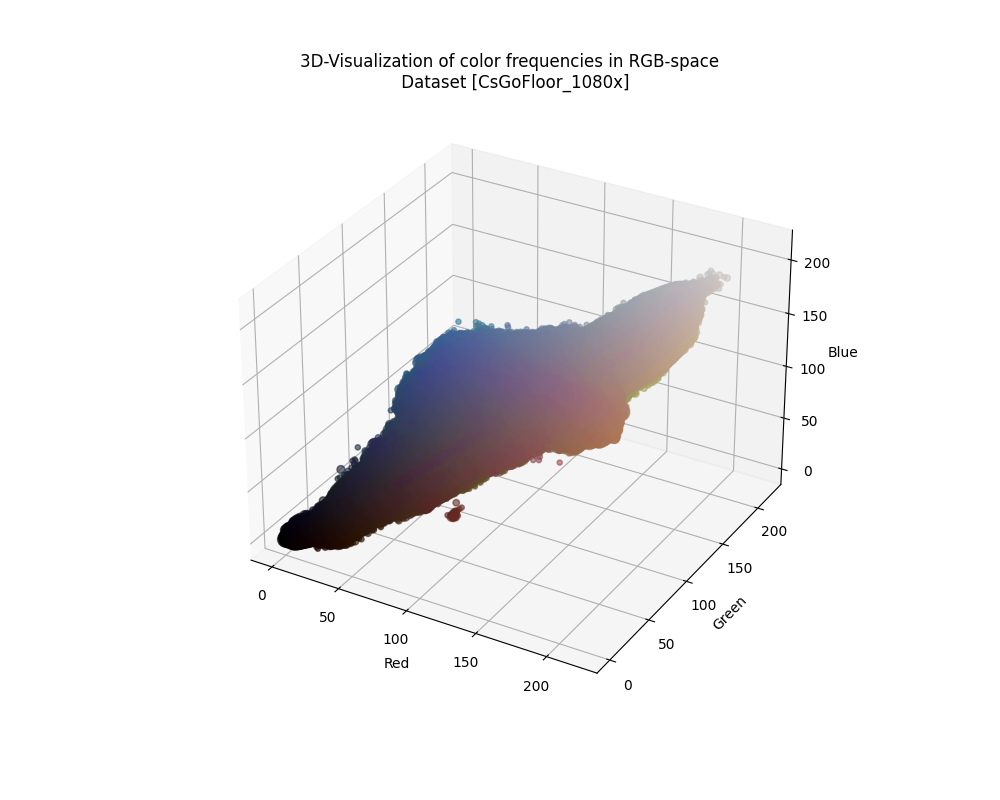
\includegraphics[width=\linewidth]{../code/dataAnalysis/output/CsGoFloor_1080x.png}
          \caption{CsGoFloor-Textures}
          \label{fig:dataset-CsGoFloor-Textures}
        \end{subfigure}%
        \hfill
        \begin{subfigure}{.33\textwidth}
            \centering
            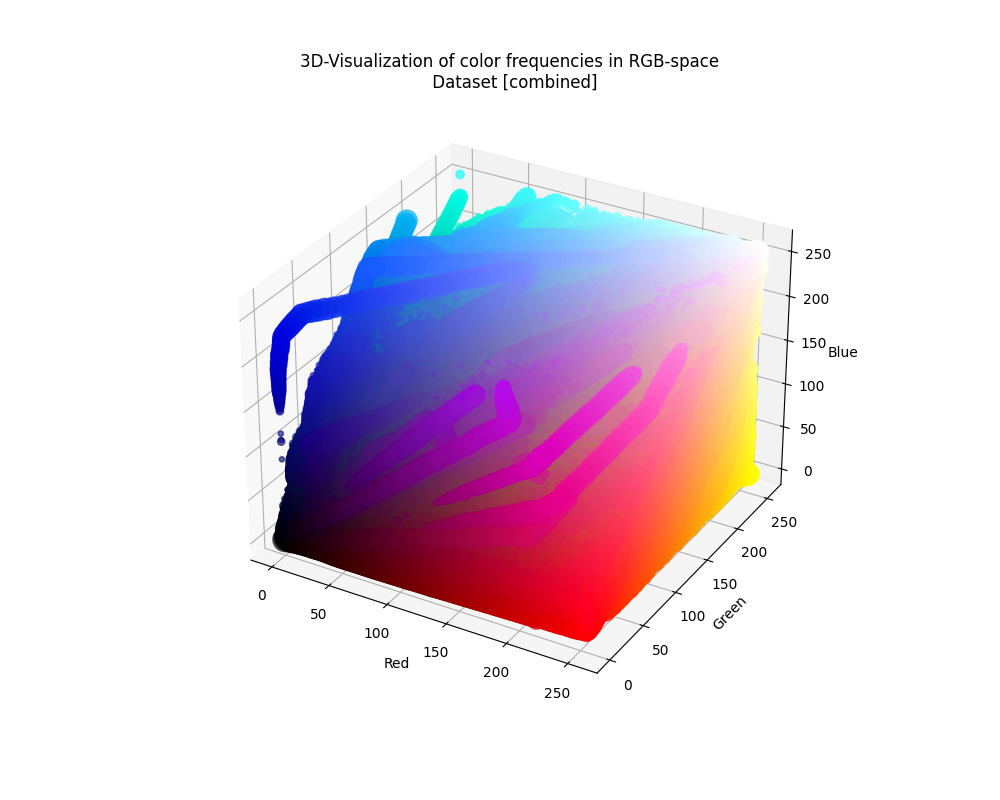
\includegraphics[width=\linewidth]{../code/dataAnalysis/output/combined.png}
            \caption{Combined}
            \label{fig:dataset-Combined}
        \end{subfigure}%
        \hfill
    \end{figure}

    In the figure above, the color distributions of the individual datasets are shown. The first five subfigures represent the color distributions of the individual datasets, while the last subfigure (\ref{fig:dataset-Combined}) shows the combined color distribution of all datasets. The color distributions of the individual datasets are quite similar, except for the Minecraft-Textures dataset, which is way more colorful than the others. The combined figure is a combination of all the individual datasets, and it is evident that the color distribution is quite diverse. This is a positive sign, as it indicates that the dataset is not focused on only a specific color spectrum.

    \subsubsection{Data Synchronization}

    In the thesis, a manual data synchronization routine is established to maintain data consistency between the supercomputer located in Berlin and the local workstation.

\subsection{Training process}
    (gpu cluster göthingen, my GPU, ...)

\subsection{Models}
    (LLMs, basic idea, roll model, spiral model)

    \subsubsection{Column Image Transformer}

    In the context of this thesis, a model termed the Column Image Transformer (CIT) has been conceptualized and developed. This model embodies an adaptation of the conventional transformer architecture. Distinctively, the CIT model diverges from traditional image processing techniques by segmenting the image into vertical slices or columns of pixels. This segmentation allows for a method where each column is processed on its own, following the "B" batch dimension in the model's structure.

    The model assigns position embeddings to every pixel in a column, indicated by the "H" dimension. This approach enables the model to predict the properties of subsequent pixels within the same column, enhancing the model's ability to reconstruct image content and have a basic understanding of the context. Each pixel includes three values corresponding to the Red, Green, and Blue (RGB) color channels. These channels are processed across the model's layers as the "C" dimension.

    \subsubsection{Spiral Image Transformer}

    The second approach is represented by the Spiral Image Transformer (SIT). Unlike its predecessor, the Column Image Transformer (CIT), the SIT model employs a contextually spiral pattern. This architecture enables the generation of images starting from a central point and expanding outward (see ...). In the SIT model, the batch dimensions correspond to distinct images, whereas the H dimension represents the spiral context. Similar to the CIT model, the C dimension denotes the color channels.

    One of the pivotal enhancements of the SIT model is its ability to analyze adjacent pixels on the horizontal axis, in contrast to the CIT model's limitation to columnar pixel analysis. This feature is particularly beneficial for interpreting textures with intricate patterns, such as diagonal ones, thereby offering an advantage over the Column Image Transformer. However, it is important to note that the SIT model operates within a constrained area of the image due to its 2D context. This limitation necessitates the use of only a portion of the image area, specifically a sector determined by the square root of the total area available to the Column Image Transformer (CIT), with an equal context length.
    
